\chapter{Curbe Eliptice} 

În aceast capitol vom prezenta conceptul de curbă eliptică, pornind de la definițiile de bază, fiind incluse concepte precum structura de grup formată de punctele de pe o curbă eliptică, construcția curbelor eliptice, reprezentări ale punctelor de pe o curbă. Vom continua discuția spre aritmetica eficientă, unde vom prezenta algorimi eficienți pentru înmulțirea unui punct cu un scalar și pentru țnmulțire multiplă, prezentând câte un exemplu la fiecare algoritm.

\section{Introducere}
\label{sec:sec01}

\begin{dfn}
Conform \cite{eccDefs}, definim o \textit{curbă eliptică} $E$ peste un corp $K$ prin ecuația:
$$E : y^2 + a_1xy + a_3y = x^3 + a_2x^{2} + a_4x + a_6$$ 
\\unde $a_1, a_2, a_3, a_4, a_5, a_6\in K$, iar discriminantul ecuației, $\Delta \neq 0$. Discriminantul ecuației este definit astfel:
$$ \begin{cases}
\Delta = -d_2^{2}d_8 - 8d_4^{3} - 27d_6^{2} + 9d_2d_4d_6 \\
d_2 = a_1^{2} + 4a_2 \\
d_4 = 2a_4 + a_1a_3 \\
d_6 = a_3^{2} + 4a_6 \\
d_8 = a_1^{2}a_6 + 4a_2a_6 - a_1a_3a_4 + a_2a_3^{2} - a_4^{2}
\end{cases}$$
\end{dfn}
\begin{dfn}
Fie $L$ orice extensie a corpului $K$. Definim mulțimea de $L$-puncte raționale peste $E$ astfel: $E(L) = \set {(x, y)\in L\times L: y^2 + a_1xy + a_3y - x^3 - a_2x^{2} - a_4x - a_6 = 0} \cup \set {\infty}$
\end{dfn}
\begin{obs}
În următoarele rânduri voi face o serie de observații asupra ecuației unei curbe eliptice: \\
(i) Ecuația de la definiția 2.1 se numește \textit{Ecuație Weierstrass} \\
(ii) Condiția ca discriminantul $\Delta$ să fie diferit de 0, asigură "netezimea" curbei eliptice, adică nu există puncte care să aibe 2 sau mai multe tangente diferite la curbă. \\
(iii) L-punctele raționale sunt acele puncte, $(x, y)$, care satisfac ecuația Weierstrass, cu $x, y \in L$. Punctul de la infinit este considerat un punct L-rațional pentru toate extensiile $L$ ale corpului $K$
\end{obs}

\begin{dfn}
Fie $E_1, E_2$ două curbe eliptice, definite astfel: \\
$E_1 : y^2 + a_1xy + a_3y = x^3 + a_2x^{2} + a_4x + a_6$ \\
$E_2 : y^2 + \overline{a_1}xy + \overline{a_3}y = x^3 + \overline{a_2}x^{2} + \overline{a_4}x + \overline{a_6} $ \\
Spunem că cele două curbe sunt \textit{izomorfe} dacă există $u,r,s,t\in K, u\neq 0$ astfel încât schimbarea de variabilă $(x, y)\rightarrow (u^2x + r, u^3y + u^2sx + t)$ transformă ecuația $E_1$ în ecuația $E_2$. Acest tip de transformare se numește schimbare "admisibilă" de variabilă.
\end{dfn}
\begin{dfn}
Ecuația Weierstrass a unei curbe eliptice poate fi simplificată în mod considerabil, aplicând schimbări admisibile de variabilă. Vom trata trei cazuri separate de schimbări de variabilă, în funcție de caracteristica corpului $K$, ajungând la o formă \textit{simplificată a Ecuației Weierstrass.}. Vom aborda trei cazuri, primul fiind $char(K) \neq \set {2,3}$ \\

  1. Fie $K$ un corp si \textit{E} o curbă eliptică dată prin ecuația lui Weierstrass. O schimbare admisibilă de variabilă este:
$(x, y) \rightarrow (\frac{x - 3a_1^{2} - 12a_2}{36}, \frac{y-3a_1x}{216} - \frac{a_1^{3} + 4a_1a_2 - 12a_3}{24})$ \\
Această schimbare transformă ecuația $E$ în ecuația 
\begin{center} $y^2 = x^3 + ax + b; a, b\in K$\end{center}
Discriminantul acestei noi ecuații este $\Delta = -16(4a^3 + 27b^2)$ \\

2. Dacă $char(K) = 2$ trebuie să considerăm două subcazuri. Dacă $a_1 \neq 0$, atunci o schimbare admisibilă de variabilă este: $(x, y) \rightarrow (a_1^2x + \frac{a_3}{a_1}, a_1^3y + \frac{a_1^2a_4 + a_3^2}{a_1^3} )$, care transformă $E$ în:
\begin{center}$y^2 + xy = x^3 + ax^2 + b; a, b\in K$\end{center}
O astfel de ecuație se numește \textit{non-supersingulară} și are discriminantul $\Delta = b$ \\
Dacă $a_1 = 0$ atunci o schimbare admisibilă ar fi $(x, y)\rightarrow (x + a_2, y)$ care transformă curba $E$ in
\begin{center} $y^2 + cy = x^3 + ax + b; a,b,c\in K$ \end{center}
O astfel de ecuație se numește \textit{supersingulară} și are discriminantul $\Delta = c^4$
\\

3. Dacă $char(K) = 3$ trebuie să considerăm din nou două subcazuri. Dacă $a_1^2 \neq -a_2$, atunci o schimbare admisibilă de variabilă este
$(x, y) \rightarrow (x + \frac{\alpha}{\beta}, y + a_1x + a_1\frac{\alpha}{\beta} + a_3)$, unde $\alpha = a_4 -a_1a_3$ și $\beta = a_1^2 - a_2$. Ecuația $E$ devine: 
\begin{center} $y^2 = x^3 + ax^2 + b; a, b\in K$\end{center}
O astfel de ecuație se numește \textit{non-supersingulară} și are discriminantul $\Delta = -a^3b$ \\
Dacă $a_1^2 = -a_2$, atunci considerăm o schimbare admisibilă de variabilă $(x, y) \rightarrow (x, y + a_1x + a_3)$, care transformă curba $E$ în:
\begin{center} $y^2 = x^3 + ax + b$ \end{center}
O astfel de curbă este \textit{supersingulară} și are discriminantul $\Delta = -a^3$
\end{dfn}

\begin{obs}
Vom lucra cu forma simplificată a ecuației Weierstrass pe tot parcursul următoarelor capitole.
\end{obs}

\subsection{Grupul punctelor de pe o curbă eliptică}
\label{subsec:subsec01}
Fie $E$ o curbă eliptică în formă Weierstrass peste un corp $F_q$. Punctele care aparțin acestei curbe formează o structură de grup abelian, acestea respectând regulile unei astfel de structuri.

\begin{itemize}
  \item Definim elementul neutru în grup ca fiind punctul de la infinit, notat $\infty$. Astfel, pentru orice punct $P$ de pe curbă, avem: $P + \infty = \infty + P$
  \item Fie $P(x, y)\in E(F_q)$. Atunci există $-P = (x, -y) \in E(F_q)$ astfel încât $P+ (-P) = \infty$. Numim $-P$, inversul punctului $P$. De asemenea, avem $\infty = -\infty$
  \item Oricare ar fi două puncte, $P, Q\in E(F_q)$, avem $P + Q \in E(F_q)$. În continuare vom defini această operație de adunare mai în detaliu.
\end{itemize}

\begin{dfn}
Adunarea a două puncte de pe o curbă eliptică este foarte intuitivă din punct de vedere geometric. Fie $P, Q$ două puncte și $R$ suma lor. Rezultatul este obținut astfel. Mai întâi desenăm o linie între $P, Q$. Acestă linie intersectează curba într-un al treilea punct. Punctul $R$ este reflecția la axa $Ox$ a acestui punct(Figura 2.1a). Dublul unui punct $P(2P = R)$ este definit astfel. Desenăm o tangentă la curba eliptică în P, aceasta intersectând curba într-un punct secundar. Punctul $R$ este din nou reflecția la axa $Ox$(Figura 2.1b).  
\end{dfn}

\begin{obs}
Formulele algebrice pentru adunarea a două puncte diferă în funcție de sistemul de coordonate folosit, sau tipul de corp algebric peste care este definită curba eliptică (corp prim, binar sau de extensie).
\end{obs}

\begin{figure}[htp]
\centering
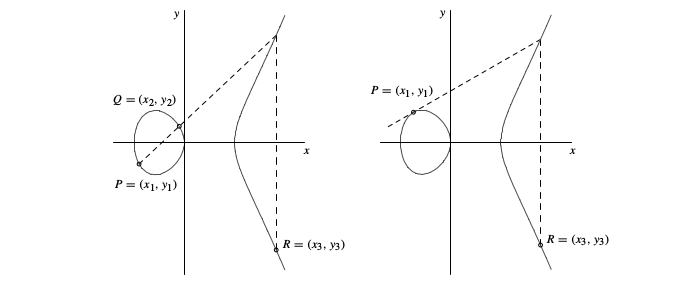
\includegraphics[width=13cm]{chapters/Addition.png}
\caption{Adunarea si dublarea unui punct pe o curba eliptica}
\label{fig:lion}
\end{figure}

\begin{dfn}
Pentru punctele reprezentate prin coordonate afine, formulele de calcul sunt după cum urmează. Fie două puncte, $P(x_{1}, y_1), Q(x_2, y_2)\in E(F_p)$. Notăm cu $R(x_3, y_3) = P + Q$. Formulele pentru adunarea a două puncte pot fi demonstrate matematic destul de ușor, pornind de la ideea ca $P, Q$ și simetricul rezultatului față de axa $Ox$ se află pe aceași dreaptă, respectiv pe aceași curba eliptică.

$\begin{cases} 
    x_3 = \lambda^2 - x_1 - x_2 \\
    y_3 =  \lambda (x_1-x_3) - y_1
   \end{cases}$
 \\cu 
 \\$
 \lambda = 
 \begin{cases}
 \frac{y_2 - y_1}{x_2 - x_1}, P \neq Q \\ 
 \frac{3x^{2}_1 + a}{2y_1}, P = Q
 \end{cases}$ \\
\end{dfn}

\begin{dem}
Fie $P(x_1, y_1), Q(x_2, y_2)\in E(F_p)$ Punctele se află pe aceași dreaptă. Scriind ecuația dreptei care trece prin cele două puncte și considerând că $-R\in E(F_p)$, rezolvăm sistemul de ecuații:
$\begin{cases} 
    0 = \begin{vmatrix}
			x_1 & y_1 & 1 \\ 
			x_2 & y_2 & 1 \\ 
			x & y & 1  \\ 
			\end{vmatrix} \\
    y^2 =  x^3 + ax + b
   \end{cases}$
   Panta dreptei este $\lambda = \begin{cases}
 \frac{y_2 - y_1}{x_2 - x_1}, P \neq Q \\ 
 \frac{3x^{2}_1 + a}{2y_1}, P = Q
 \end{cases}$
 \\Înlocuind în formula curbei eliptice, obținem formulele din definiția precedentă.
\end{dem}

\subsection{Construcția curbelor eliptice}
\label{subsec:subsec02}

Fie $E$ o curbă eliptică peste un corp $K = F_q$. Așa cum am văzut în secțiunea anterioară, mulțimea de puncte $E(F_q)$ împreună cu operația de adunare, formează o structură de grup abelian, cu punctul de la infinit fiind elementul neutru din grup. Acest grup este folosit în criptografia bazată pe curbe eliptice.


\begin{dfn}
Numim \textit{ordin} al unei curbe eliptice, numărul de puncte care satisfac ecuația Weierstrass, cu alte cuvinte, cardinalul mulțimii $E(F_q)$ și il notăm cu $\# E(F_q)$. Teorema care urmează, datorată lui \textit{Hasse}, oferă o aproximare pentru acest ordin
\end{dfn}
\begin{teo}
Fie $E$ o curbă eliptică definită peste $F_q$. Atunci este adevărată relația:
\begin{center} $q + 1 - 2\sqrt{q}\leq \# E(F_q)\leq q+1 + 2\sqrt{q}$ \end{center}
Întrucât $2\sqrt{q}$ este relativ mic în comparație cu $q$, putem afirma că $\# E(F_q) \approx q$
\end{teo}
\begin{teo}
Fie $q = p^m$, unde $p$ este caracteristica corpului $F_q$. Atunci există o curbă eliptică $E$ definită peste acest corp, cu $\# E(F_q) = q+1-t$ ($t$ se numește urma curbei eliptice $E$) dacă și numai dacă una dintre următoarele condiții este adevărată: \\
(i) $t \not\equiv 0$ mod $p$ si $t^2\leq 4q$ \\
(ii) m este impar și $t=0$ sau $t^2 = 2q$ și $p=2$ sau $t^2 = 3q$ și $p=3$ \\ 
(iii) m este par și $t^2 = 4q$ sau $t^2 = q$ și $p\not\equiv 1$ mod $3$ sau $t= 0$ și $p\not\equiv 1$ mod $4$
\end{teo}
\begin{dfn}
Fie $p$ caracteristica corpului $F_q$. Numim curbă eliptică \textit{supersingulară}, dacă $p$ divide $t$, unde t este urma curbei. Altfel, curba $E$ este \textit{non-supersingulară}
\end{dfn}
\begin{teo}
Fie $E$ o curbă eliptică peste corpul $F_q$ și fie ordinul acesteia $\# E(F_q)= q+ 1-t$. Atunci, $\# E(F_q) = q+ 1 - V_n$, unde definim șirul $\set {V_n}$ recursiv, prin formula $V_0 = 2, V_1=t$ și $V_n = V_1V_{n-1} - qV_{n-2}, \forall n\geq 2$
\end{teo}
Următoarea teoremă, descrie structura grupului pentru o curbă eliptică. Vom nota un grup ciclic de ordin n, cu $Z_n$.
\begin{teo}
Fie E o curbă eliptică definită peste $F_q$. Atunci grupul $E(F_q)$ este izomorfic cu $Z_{n_1} \oplus Z_{n_2}$, unde $n_1, n_2\in Z$, unici determinati, cu $n_2$ care divide atât $n_1$ cât și $q-1$. Dacă $n_2=1$, spunem ca $E(F_q)$ este grup ciclic.
\end{teo}

\subsection{Reprezentări ale punctelor de pe o curbă eliptică}
\label{subsec:subsec03}
De multe ori, în efectuarea operațiilor pe curbe eliptice, poate fi avantajos să reprezentăm un punct, în alte coordonate decât cele afine. De exemplu, în calculul sumei a două puncte (operație care la rândul ei este folosită în algoritmii pentru înmulțirea cu un scalar și în înmulțirea multiplă) se observă necesitatea de a efectua operația de invers modular de mai multe ori. Acestă operație este costisitoare din punct de vedere computational, astfel vom folosi diferite tipuri de reprezentări.
\begin{dfn}
Fie $K$ un corp și $c, d\in \mathbb{N}$. Definim o relație de echivalență peste mulțimea $K^3\setminus \set {(0, 0, 0)}$ ca fiind :
\begin{center} $(X_1, Y_1, Z_1) \equiv (X_2, Y_2, Z_2)$ dacă $X_1 = \lambda ^cX_2, Y_1 = \lambda ^d Y_2, Z_1 = \lambda Z_2, \lambda\in K^{*}$\end{center}
Există o corespondență $1-1$ între mulțimea de puncte în coordonate proiective $P(K)^{*} = \set {(X, Y, Z): X, Y, Z\in K, Z\neq 0}$ și mulțimea punctelor în coordonate afine, $A(K) = \set {(x, y): x, y\in K}$
\end{dfn}
\begin{dfn}
Considerăm $c=1, d=1$ în definiția \textit{coordonatelor proiective}. Acestea se numesc \textit{coordonate proiective standard}. Punctul l în coordonate proiective $(X, Y, Z), Z\neq 0$ corespunde punctului în coordonate afine $(X/Z, Y/Z)$. Ecuația curbei eliptice devine:
\begin{center}  $Y^2Z = X^3 + aXZ^2 + bZ^3$ \end{center}
Punctul de la infinit este $(0, 1, 0)$ în timp ce inversul unui punct oarecare este $(X, -Y, Z)$
\end{dfn}
\begin{dfn}
Considerăm $c=2, d=3$. Acest sistem de coordonate se numesc coordonate \textit{proiective Jacobi}. Punctul $(X, Y, Z), Z\neq 0$ corespunde punctului 
în coordonate afine $(X/Z^2, Y/Z^3)$. Ecuația curbei devine:
\begin{center} $Y^2 = X^3 + aXZ^4 + bZ^6$ \end{center}
Punctul de la infinit este $(1, 1, 0)$, iar inversul unui punct este $(X, -Y, Z)$
\end{dfn}
\begin{dfn}
\textit{Coordonatele Chudnovsky} sunt obținute din coordonatele Jacobi, adăugând niște redundanțe. Astfel, un punct reprezentat în acest tip de coordonate, arată în acest fel: $(X, Y, Z, Z^2, Z^3)$. Acest tip de reprezentare aduce îmbunătățiri de performanță când folosim anumiți algoritmi specializați pentru înmulțirea cu un scalar.
\end{dfn}

\begin{obs}
Se poate folosi $Z = 1$ in implementări pentru a simplifica calculele.
\end{obs}

\section{Aritmetică eficientă}
\label{sec:sec02}

În această secțiune vom face o prezentare a metodelor eficiente de înmulțire cu un scalar și de înmulțire multiplă. Printre metodele de înmulțire cu un scalar, se numără algoritmul binar, algoritmul care folosește o reprezentare cu semn a scalarului și diferite metode de înmulțire cu fereastră. La înmulțirea multiplă, avem un algoritm naiv si două metode de înmulțire eficientă. 

\subsection{Inmulțirea cu un scalar}

\begin{dfn}
Definim operația de înmulțire a unui punct $P$ de pe o curbă eliptică, cu un scalar, $k\in \mathbb{Z}$, notată cu $kP$, ca fiind: \\
- $0P = \infty$ \\
- $(k+1)P = kP + P, k\geq 0$ \\
- $kP = -|k|P, k < 0$ \\
Există multe metode de a face acest lucru, de la metoda \textit{brute force}, care face k adunări repetate ($kP = P+P+\cdots +P$) până la metode mai rafinate, precum cea a ferestrei glisante, care îmbunătățesc considerabil performanța operației. Vom discuta în continuare despre diferite metode eficiente pentru această operație.
\end{dfn}

\subsubsection{Metoda Binară}

Metoda naivă de a înmulți un punct cu un scalar, cea prezentată in definiție, necesită $k-1$ adunări pentru a calcula $kP$. O primă optimizare este dată de această metoda binară, care necesită cel mult $m$ adunări \cite{binary} și în medie $m/2$ adunări, unde $m$ este numărul de biți din reprezentarea lui $k$. Algoritmul constă în procesarea de la dreapta la stânga, sau de la stânga la dreapta a scalarului. După fiecare bit parcurs, dublăm rezultatul și când întâlnim un bit de $1$ adunăm punctul $P$ la rezultat. Astfel, după parcurgerea a $\log_2 k$ iterații(numărul de biți din reprezentarea lui $k$) avem rezultatul.

\begin{ex}
Fie curba eliptică $E: y^2 = x^3 + 3x + 2$, punctul $P(10, 16)\in E$ și un scalar $d = 5$. Reprezentarea binară a scalarului este $d = (1, 0, 1)$. Așadar rezultatul va fi egal cu: $r = (10, 16) + 4*(10, 16)$. Am adunat la rezultat $P$, deoarece cel mai nesemnificativ bit este 1, apoi am dublat $P$ de 2 ori(2 biți parcurși) și l-am adunat la rezultat deoarece bitul cel mai semnificativ este $1$. Astfel obținem $5P = (66, 73)$
\end{ex}

\subsubsection{Reprezentări cu semn}

Un avantaj major al curbelor eliptice, este faptul că în grupul format de punctele de pe o astfel de curbă, operația de invers este foarte eficientă. Astfel, dacă consideram 2 puncte $P, Q$ într-un astfel de grup, putem calcula $P + Q$ si $P - Q$ cu aproximativ același cost computațional. Această observație este foarte importantă în eficientizarea algoritmilor de înmulțire cu un scalar. Calculul inversului, având un cost neglijabil din punct de vedere computațional, nu este necesar să ne limităm la $\set{0, 1}$ în reprezentarea unui scalar. Introducem astfel, conceptul de reprezentare cu semn.

\begin{dfn}
Conform, \cite{solinas}, o reprezentare a lui $n\in\mathbb{N}$, cu semn, poate fi notată astfel: $n = <u_{l-1}u_{l-2}...u_1u_0>$, unde $u_i\in\set{0, -1, 1}$. Astfel $n = \sum_{i=0}^{l-1} u_i 2^{i}$. Există o infinitate de astfel de reprezentări.
\end{dfn}
\begin{dfn}
Reprezentarea cu semn optimă pentru operația de înmulțire cu un scalar este așa numita NAF, sau Non Adjacent Form. Aceasta are proprietatea ca nu există două elemente consecutive din reprezentarea cu semn diferite de 0.
\end{dfn}

\begin{teo}
NAF-ul are urmatoarele proprietati:
\begin{itemize}
  \item Orice număr natural are un NAF
  \item NAF-ul unui număr este unic
  \item Lungimea NAF-ului unui număr natural este cu cel mult o unitate mai mare decât expansiunea binară a numarului 
  \item NAF-ul are distanța Hamming minimă dintre toate reprezentările cu semn
\end{itemize}
\end{teo}

Un algoritm care folosește această reprezentare a scalarului, funcționează asemănător cu cel de la metoda binară. Parcurgem reprezentarea cu semn, dublăm rezultatul după fiecare bit parcurs, adunăm $P$ când întâlnim un bit de $1$ și scădem $P$ când întâlnim un bit de $-1$. Această metodă necesită în medie $m/3$ adunări și $m$ dublări, unde m reprezintă numărul de biți din reprezentarea scalarului \cite{nafCost}.

\begin{ex}
Fie curba eliptică $E: y^2 = x^3 + 3x + 2$, punctul $P(10, 16)\in E$ și un scalar $d = 5$. Reprezentarea cu semn a lui d este, $d = (1, 0, 0, -1)$. Parcurgem de la dreapta la stânga rezultatul și avem după prima iterație $rezultat = P$. După a doua iterație $resultat = 2P$. Dupa a treia iterație $rezultat = 4P$, iar la ultima iterație, $rezultat= 8P - P= 7P$. Așadar $7P = (14, 13)$
\end{ex}

\subsubsection{Metoda cu fereastră}

Algoritmii care se folosesc de reprezentarea cu semn a scalarului pot fi îmbunătățiți dacă avem disponibilă mai multă memorie. Vom procesa $w$ cifre din scalar la o iterație, unde $w$ reprezintă lățimea ferestrei.

\begin{dfn}
Fie $w\geq 2$ un număr natural. Numim o reprezentare NAF de lățime $w$ pentru un scalar $n\in\mathbb{N}$, notată cu $w-NAF$, un șir de numere $n = <u_{l-1}u_{l-2}...u_1u_0>$ astfel încât $|u_i| < 2^{w-1}$ și $n = \sum_{0}^{l-1}u_i2^i$ astfel încât cel mult una din $w$ cifre consecutive din șir este diferită de 0.
\end{dfn}

\begin{teo}
Următoarele proprietăți sunt adevarate pentru $w-NAF$:
\begin{itemize}
\item $2-NAF = NAF$ pentru orice număr $k\in\mathbb{N}$
\item $w-NAF$ unui număr este unic
\item Reprezentarea $w-NAF$ este cu cel mult un bit mai mare decât reprezentarea binară a unui număr
\item Densitatea medie a cifrelor diferite de $0$ din reprezentarea $w-NAF$ de lungime $l$ a unui număr este $\frac{1}{w+1}$
\end{itemize}
\end{teo}

Algoritmul care calculează $nP$ folosind această metodă, este asemănător cu algoritmii precedenți, dar folosim această reprezentare $w-NAF$ pentru scalar. Fie $n = <u_{l-1}u_{l-2}...u_1u_0>$ reprezentarea $w-NAF$ a unui număr natural $n$. Dorim să calculam $nP$. Algoritmul nostru parcurge fiecare număr din reprezentarea $w-NAF$, dublând rezultatul după fiecare iterație, adunând sau scăzând $u_iP$ la rezultat, $i\in \set{0, l-1}$. Valoarea lui $u_iP$ este precalculată și stocată. \\

Conform teoremei $2.6$, numărul mediu de adunări și dublări pentru algoritmul prezentat mai sus este $[1D + (2^{w-2} - 1) A] + [\frac{m}{w+1}A + mD]$, unde $m = \log_2 n$, $A$ reprezintă adunare și $D$ dublare. \cite{windowCost}

\begin{ex}
Fie curba eliptica $E: y^2 = x^3 + 3x + 2$, punctul $P(10, 16)\in E$, un scalar $d = 39$ și lățimea ferestrei $w=3$. Reprezentarea $3-NAF$ pentru d este $(1, 0, 0, -3, 0, 0, -1)$. Vom precalcula și stoca valorile pentru $(P, 3P)$, iar apoi parcurgem $3-NAF$ de la stânga la dreapta. Inițializăm variabila rezultat cu "punctul de la infinit", iar după fiecare iteratie, în rezultat vom avea: $P, 2P, 4P, 5P, 10P, 20P, 39P$. După fiecare bit parcurs, am dublat rezultatul, am scăzut $-3P$ la iterația 4 și $-P$ la ultima iterație. Ambele valori erau precalculate. La final, avem $rezultat = 39P = (60, 39)$
\end{ex}

\subsubsection{Metoda cu fereastră glisantă}

    Pentru a eficientiza metoda cu fereastră fixă prezentată mai sus, vom folosi o așa zisă "fereastră glisantă" asupra cifrelor din $w-NAF$. Ideea e să folosim o fereastră de lățime $w$ pe care o "glisăm" (sărim peste cifrele consecutive de $0$) peste reprezentarea scalarului. Menținem întotdeauna o valoare impară în fereastră pentru a micșora numărul de precalculari necasar. La fiecare iterație, când găsim o cifra diferită de $0$ în $w-NAF$, căutăm cel mai mare $t \leq w$ astfel încât valoarea numărului dat de $w-NAF$ de lungime t este impară. Adunăm sau scădem la rezultat acea valoare apoi "glisăm" fereastra la dreapta cu $t$ poziții.
\begin{obs}
Conform \cite{slidingCost}, numărul mediu de zerouri între ferestre este egal cu:
$$\nu(w) = \frac{4}{3} - \frac{(-1)^w}{3\times 2^{w-2}}$$
Astfel, numărul mediu de adunări și dublări al algoritmului cu fereastră glisantă este:
$$[1D + (\frac{2^w - (-1)^w}{3} - 1)A] + \frac{m}{w + \nu(w)}A + mD$$
\end{obs}

\begin{ex}
Vom folosi același exemplu ca la Metoda cu fereastră fixă, aceași curbă, aceeași lățime a ferestrei, același punct și același scalar. Algoritmul îl aplicam de la stânga la dreapta pe $3-NAF$-ul punctului $P$. La fiecare iterație avem nevoie de o variabilă $t$ care dă dimensiunea ferestrei, și $u$, valoarea în fereastră. După fiecare iterație, vom avea: $s=1, u=1, resultat=P; resultat = 2P; resultat = 4P; s=4, u=-3, resultat = 5P; resultat = 10P; resultat = 20P; s=6, u=-1, resultat=39P$. La final, avem $39P = (60, 39)$
\end{ex}

\subsection{Înmulțirea multiplă}

\begin{dfn}
O operație asemănătoare celei de înmulțire cu un scalar, este cea de înmulțire multiplă cu scalari. Fie doua puncte, $P, Q$ de pe o curbă eliptică și doi scalari, $k, l\in \mathbb{Z}$. Dorim să aflăm rezultatul $kP + lQ$. Evident, similar cu operația de înmulțire cu un scalar, putem aplica o metodă directă de a înmulți punctul $P$ cu scalarul $k$ respectiv punctul $Q$ cu scalarul $l$ și apoi facem o adunare de puncte. Acest lucru este însă ineficient, întrucât există și aici metode mai rapide de a calcula acest lucru. Această operație de înmulțire rapidă, este una extrem de folosită în criptografia pe curbe eliptice, facându-și apariția, de exemplu, în cadrul unor protocoale criptografice, precum ECDSA, iar implementarea ineficientă a acesteia duce la mari probleme de performanță. 
\end{dfn}

\subsubsection{Metoda naivă}
O primă metodă de a aborda calculul $kP + lQ$ se bazează pe metode deja discutate. Calculăm separat $kP$ si $lQ$, folosind unii din algoritmii precizați la secțiunea anterioară, apoi adunăm rezultatele. Această metodă este ineficientă, făcând multe adunări și dublări redundante.
\begin{ex}
Fie doua puncte, $P(10, 16), Q(14, 13)\in E$, unde $E: y^2 = x^3 + 3x + 2$. Căutăm rezultatul $5P + 6Q$. Folosim metoda binara pentru a gasi resultatele $5P = (66, 73)$ și
$6Q = (89, 57)$. Apoi facem adunarea $(66, 73) + (89, 57) = (36, 20)$
\end{ex}

\subsubsection{Reprezentarea Joint Sparse Form}

\begin{dfn}

Considerăm 2 reprezentări cu semn pentru scalarii care apar în calculul $kP + lQ$. Combinăm aceste 2 reprezentări într-o singură reprezentare, pe care o vom numi reprezentare reunită. Astfel, dacă considerăm 2 reprezentări cu semn pentru $k, p$, ca fiind $<u_{l-1}u_{l-2}...u_1u_0>$ respectiv $<v_{l-1}v_{l-2}...v_1v_0>$, reprezentarea lor reunită este $(<u_{l-1}u_{l-2}...u_1u_0>, <v_{l-1}v_{l-2}...v_1v_0>)$. Există multe astfel de reprezentări, dar cea mai eficientă este așa numita Joint Sparse Form, introdusă de \cite{solinas}, care are următoarele proprietăți:
\begin{itemize}
\item Pentru oricare 3 poziții consecutive, cel puțin una este $0, 0$. Altfel spus, oricare ar fi $i, j\in\mathbb{N}$ avem $u_{i, j+k} = u_{1-i, j+k} = 0, k=0,\pm 1$
\item Termeni adiacenți nu pot avea semne diferite. Astfel, nu putem avea egalitatea $u_{i, j+1}u_{i, j} = -1$
\item Daca $u_{i, j+1}u_{i, j}\neq 0 \Rightarrow u_{1-i, j+1} = \pm 1$ si $u_{1-i, j}=0$
\end{itemize}
\end{dfn}

\begin{ex}
Fie scalarii $21, 26$. Reprezentarea lor Joint Sparse Form este dată de:
$$<1, 0, -1, 0, -1, -1>$$
$$<1, 0, -1, 0, 1, 0>$$
\end{ex}

Algoritmul care folosește această reprezentare se numește \textit{"Shamir's Trick"} și calculează $kP + lQ$ astfel. Precalculează $P, Q, -P, -Q, P + Q, P - Q, -P - Q$ și în funcție de cifrele care apar în parcurgerea reprezentării Joint Sparse, adaugă la rezultat una din valori. De exemplu dacă la o iterație avem combinația $1, 1$ adăugăm $P + Q$, dacă avem $-1, -1$ adăugăm $-P - Q$, etc. În continuare vom prezenta un exemplu de calcul cu acest algoritm.

\begin{ex}
Fie curba eliptică și punctele de la exemplul precedent, dar de această dată vom alege scalarii $d = 21, l = 26$. Vrem așadar să calculăm rezultatul $dP + lQ$ folosind metoda Joint Sparse Form. Mai întâi trebuie sa calculăm JSF pentru cei doi scalari, rezultatul fiind $(1, 0, -1, 0, -1, -1), (1, 0, -1, 0, 1, 0)$. Vom crea o variabilă $rezultat$ în care, la fiecare iterație vom avea următoarele: $rezultat = P + Q; rezultat = 2P + 2Q; rezultat = 3P + 3Q; rezultat = 6P + 6Q; rezultat = 11P + 13Q; rezultat = 21P + 26P = (48, 35)$.

\end{ex}

\subsubsection{Metoda cu fereastră intercalată, w-NAF}

Spre deosibire de metada precedentă de calcul, ideea aici este să facem pentru fiecare punct în parte precalculul separat, dar pasul de dublare trebuie făcut simultan. Putem folosi ferestre de dimensiuni diferite pentru fiecare scalar în parte, calculând $w-NAF$ lor. În faza de precalcul, stocăm pentru fiecare punct $iP, i<2^{w-1}$, $i$ impar. Reprezentările $w-NAF$ ale punctelor sunt procesate simultan de la stânga la dreapta, cu o singură variabilă $Q$ pe post de rezultat, care se dublează la fiecare iterație. Putem vizualiza ce se întâmplă cu această variabilă la fiecare iterație  în figura 2.2.

\begin{figure}[htp]
\centering
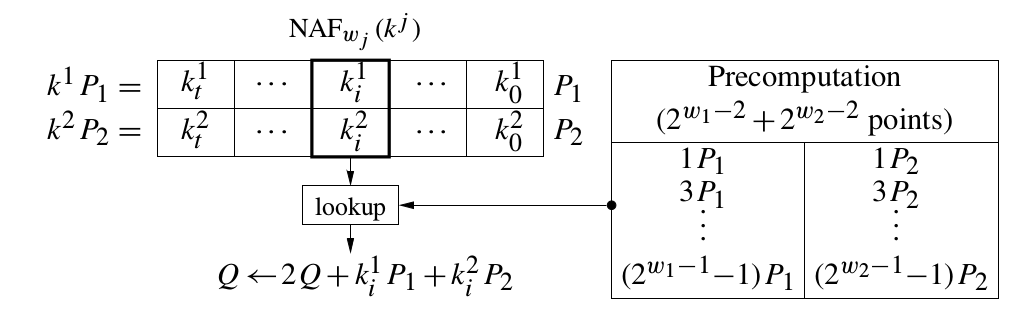
\includegraphics[width=10cm]{chapters/interleaving.png}
\caption{Variabila rezultat la o iterație oarecare}
\label{fig:lion}
\end{figure}

\begin{obs}

Conform \cite{interleaving} Numărul mediu de adunari si dublări este:
$$[|\set{j:w_j>2}|D+\sum_{j=1}^{2}(2^{w_j-2}-1)A]+[\max_{1\leq j\leq 2} l_jD + \sum_{j=1}^{2}\frac{l_j}{w_j+1}A]$$
\end{obs}

\begin{ex}
Păstrând curba și punctele de la exemplele precedente, dorim să calculăm $10P + 41Q$, cu ferestrele $4, 4$. Trebuie așadar să calculam $4-NAF$ pentru cei doi scalari. Obținem $(5, 0), (3, 0, 0, 0, -7)$. Padăm cu 0 astfel încât cele două reprezentări să aibă lungimi egale, obținând astfel $(0, 0, 0, 5, 0), (3, 0, 0, 0, -7)$. După fiecare iterație, în variabila $rezultat$ avem: $rezultat = 3Q; rezultat = 6Q, rezultat=12Q, rezultat = 5P + 24Q; rezultat = 10P + 41Q = (8, 21)$.
\end{ex}




